
\section{Einbau Kfz}
\label{section:einbau_kfz}
\begin{frame}%STARTCONTENT

\begin{columns}
    \begin{column}{0.48\textwidth}
    
\begin{figure}
    \includegraphics[width=0.85\textwidth]{foto/75}
    \caption{\scriptsize Einbau des Bedienteils eines VHF/UHF-Funkgerätes in die Mittelkonsole eines PKW}
    \label{n_mobilfunkgeraet}
\end{figure}

    \end{column}
   \begin{column}{0.48\textwidth}
       \begin{itemize}
  \item Wähend der Fahrt mit anderen Funkamateuren unterhalten
  \item Tipps oder Verkehrsinformationen mitbekommen
  \item Benutzung nur mit Freisprecheinrichtung
  \end{itemize}

   \end{column}
\end{columns}

\end{frame}

\begin{frame}
\frametitle{Einbau}
\begin{columns}
    \begin{column}{0.48\textwidth}
    
\begin{figure}
    \includegraphics[width=0.85\textwidth]{foto/64}
    \caption{\scriptsize Magnetfußantenne auf Fahrzeugdach}
    \label{n_magnetfussantenne}
\end{figure}
\begin{itemize}
  \item Groundplane-Antenne mit Fahrzeugdach als Gegenelement
  \end{itemize}

    \end{column}
   \begin{column}{0.48\textwidth}
       \begin{itemize}
  \item Möglichst mittig auf dem metallischen Fahrzeugdach
  \item Vorgaben des Fahrzeugherstellers beachten
  \item Leitungen so kurz wie möglich und entfernt von anderen Fahrzeugleitungen
  \end{itemize}

   \end{column}
\end{columns}

\end{frame}

\begin{frame}
\frametitle{Achtung}
\begin{columns}
    \begin{column}{0.48\textwidth}
    
\begin{figure}
    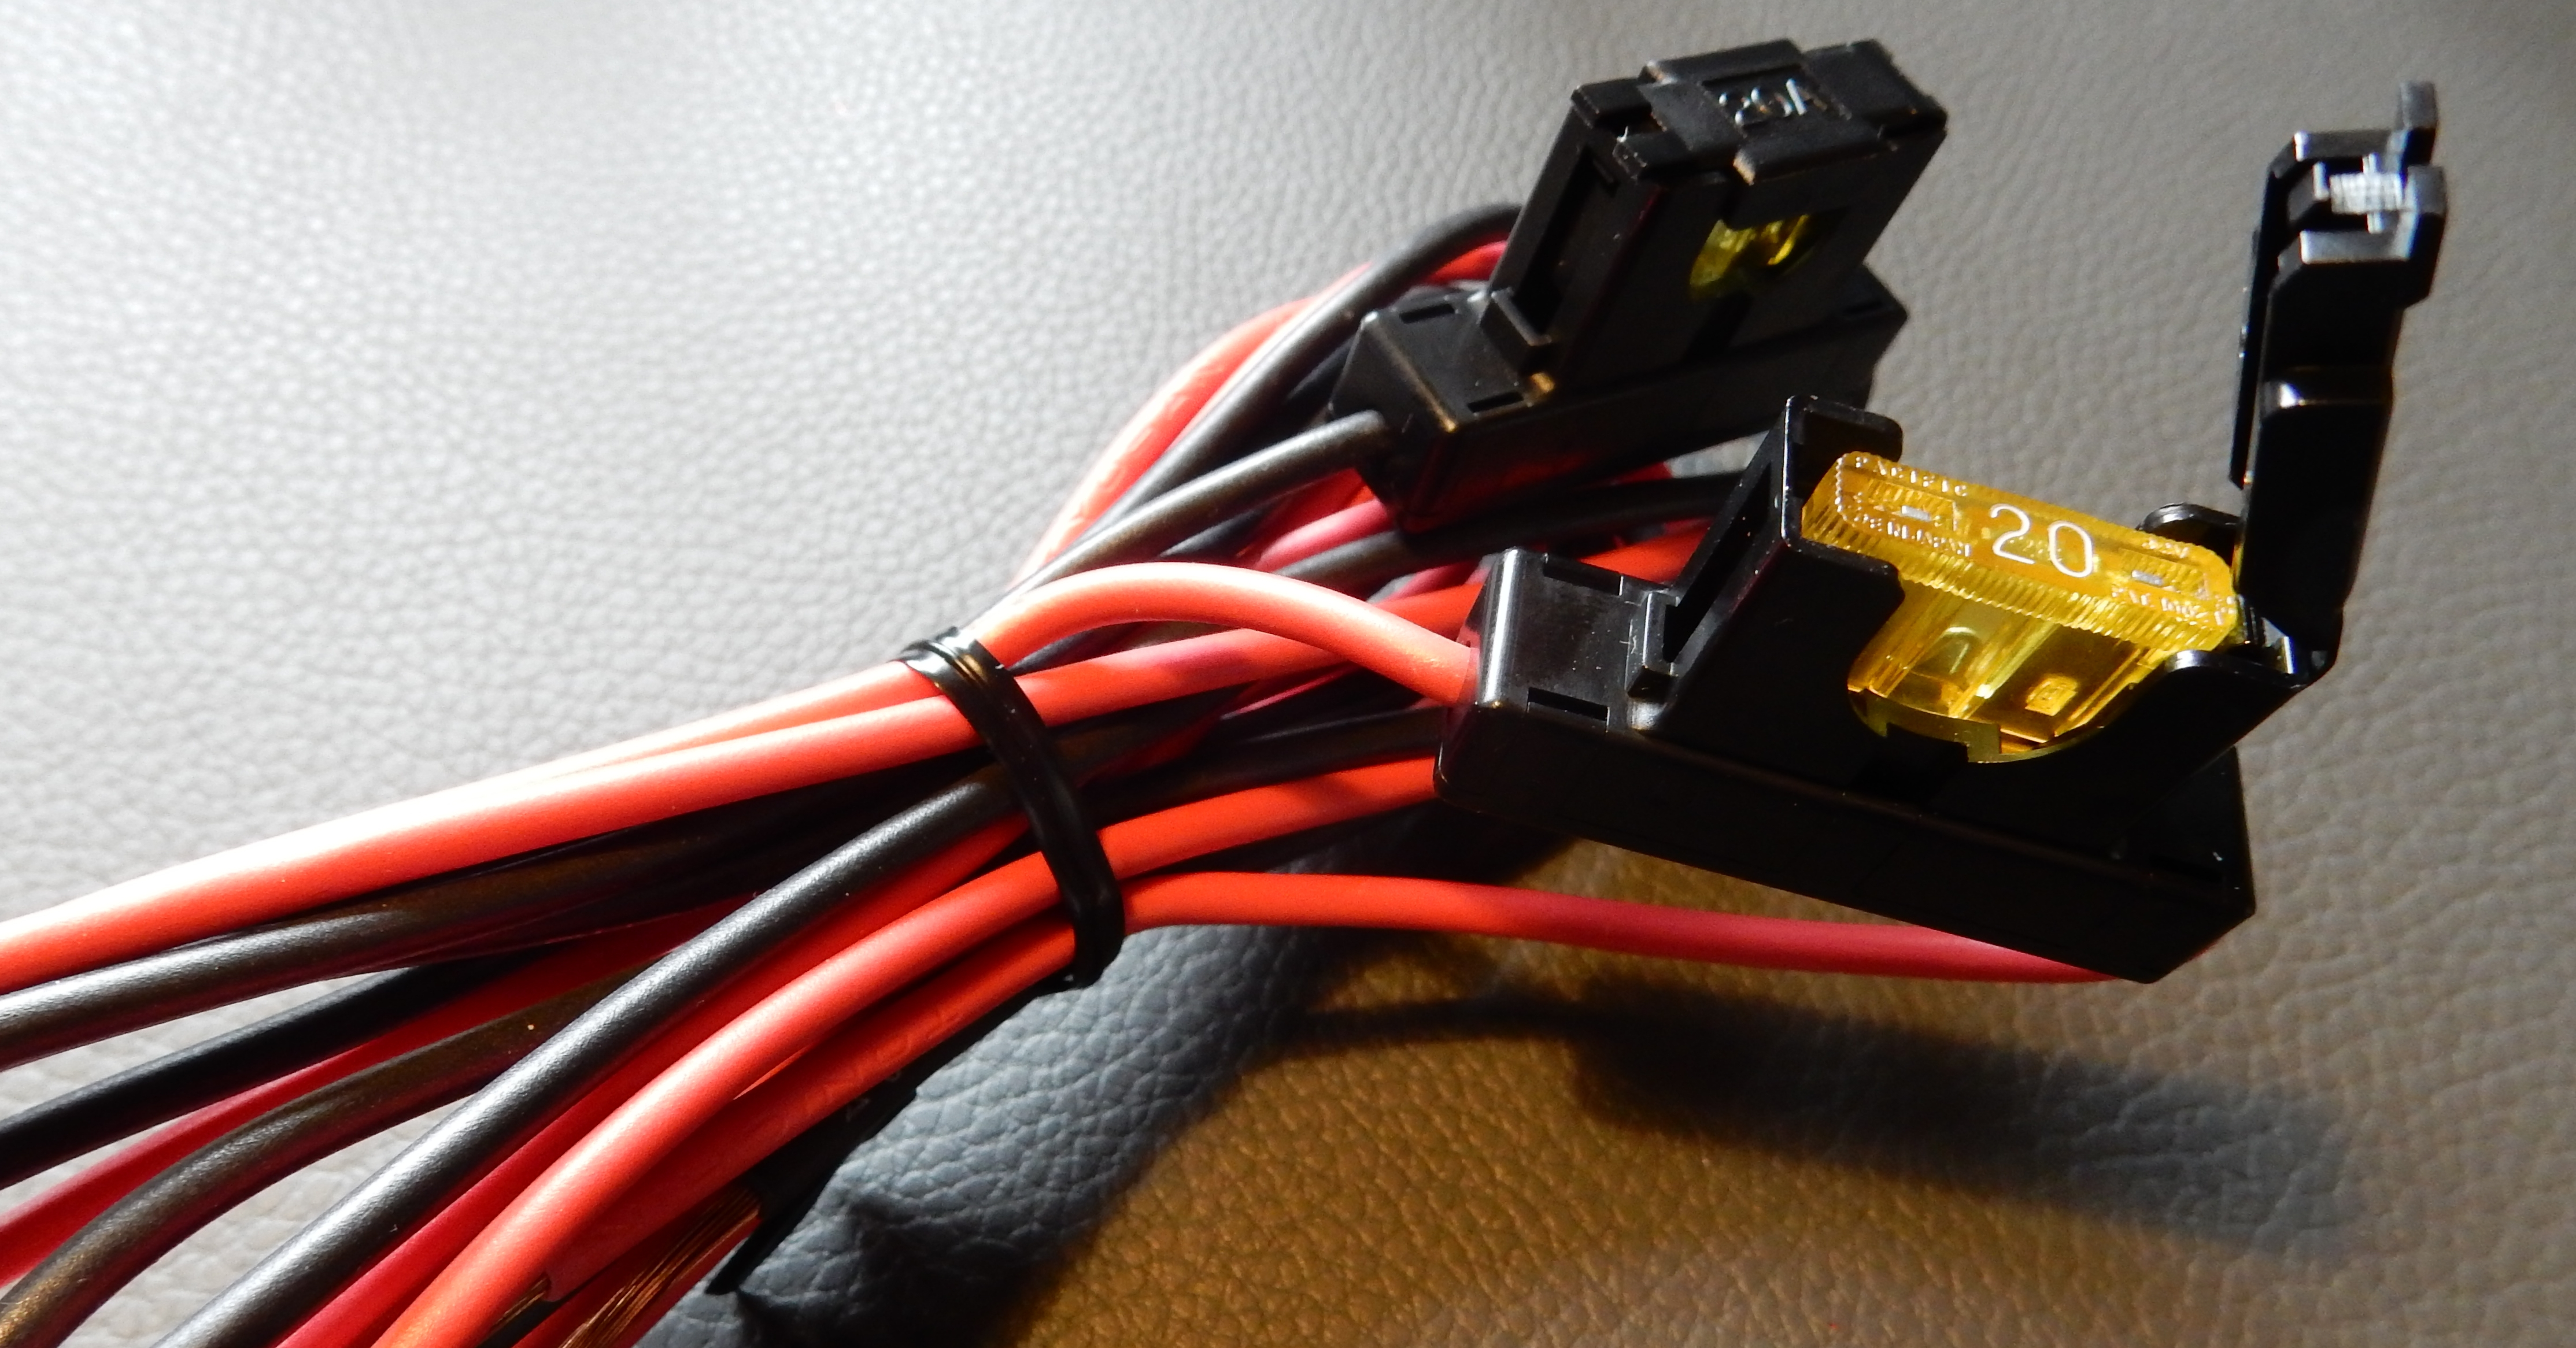
\includegraphics[width=0.85\textwidth]{foto/76}
    \caption{\scriptsize Stromkabel mit Sicherungshalter}
    \label{n_Kabelsicherung}
\end{figure}

    \end{column}
   \begin{column}{0.48\textwidth}
       \begin{itemize}
  \item Bordnetzspannung von \qty{12}{\volt} oder \qty{24}{\volt} scheint ungefährlich
  \item Hohe Ströme sind möglich
  \item Bei Kurzschluss sind Lichtbogen, Kabelbrand oder Fahrzeugbrand möglich
  \item Sicherung des richtigen Werts für das Funkgerät verbauen
  \end{itemize}

   \end{column}
\end{columns}

\end{frame}

\begin{frame}
\only<1>{
\begin{QQuestion}{NK308}{Damit die Zulassung eines Kraftfahrzeugs nicht ungültig wird, sind vor dem Einbau einer mobilen Sende-/Empfangseinrichtung grundsätzlich die Anweisungen~...}{des Amateurfunkgeräte-Herstellers zu beachten.}
{für den Einbau mobiler Sendeanlagen der Bundesnetzagentur einzuhalten.}
{des Kraftfahrt-Bundesamtes einzuhalten.}
{des Kfz-Herstellers zu beachten.}
\end{QQuestion}

}
\only<2>{
\begin{QQuestion}{NK308}{Damit die Zulassung eines Kraftfahrzeugs nicht ungültig wird, sind vor dem Einbau einer mobilen Sende-/Empfangseinrichtung grundsätzlich die Anweisungen~...}{des Amateurfunkgeräte-Herstellers zu beachten.}
{für den Einbau mobiler Sendeanlagen der Bundesnetzagentur einzuhalten.}
{des Kraftfahrt-Bundesamtes einzuhalten.}
{\textbf{\textcolor{DARCgreen}{des Kfz-Herstellers zu beachten.}}}
\end{QQuestion}

}
\end{frame}

\begin{frame}
\only<1>{
\begin{QQuestion}{NK310}{Wo sollte aus funktechnischer Sicht eine mobile VHF-Antenne an einem PKW vorzugsweise installiert werden?}{Auf der hinteren Stoßstange}
{Auf der Mitte des Metalldaches}
{Auf dem vorderen Kotflügel}
{Auf dem Armaturenbrett}
\end{QQuestion}

}
\only<2>{
\begin{QQuestion}{NK310}{Wo sollte aus funktechnischer Sicht eine mobile VHF-Antenne an einem PKW vorzugsweise installiert werden?}{Auf der hinteren Stoßstange}
{\textbf{\textcolor{DARCgreen}{Auf der Mitte des Metalldaches}}}
{Auf dem vorderen Kotflügel}
{Auf dem Armaturenbrett}
\end{QQuestion}

}
\end{frame}

\begin{frame}
\only<1>{
\begin{QQuestion}{NK309}{Um eine Beeinflussung der Elektronik des Kraftfahrzeugs zu verhindern, sollte das Antennenkabel~...}{nicht parallel und möglichst weit von der Fahrzeugverkabelung entfernt verlegt werden.}
{im Kabelbaum des Kraftfahrzeugs geführt werden.}
{über das Fahrzeugdach verlegt sein.}
{entlang der Innenseite des Motorraumes verlegt werden.}
\end{QQuestion}

}
\only<2>{
\begin{QQuestion}{NK309}{Um eine Beeinflussung der Elektronik des Kraftfahrzeugs zu verhindern, sollte das Antennenkabel~...}{\textbf{\textcolor{DARCgreen}{nicht parallel und möglichst weit von der Fahrzeugverkabelung entfernt verlegt werden.}}}
{im Kabelbaum des Kraftfahrzeugs geführt werden.}
{über das Fahrzeugdach verlegt sein.}
{entlang der Innenseite des Motorraumes verlegt werden.}
\end{QQuestion}

}
\end{frame}

\begin{frame}
\only<1>{
\begin{QQuestion}{NK307}{Welche Gefahren können beim unsachgemäßen Anschließen eines Funkgerätes an die \qty{12}{\V}-Batterie in einem Kraftfahrzeug entstehen?}{Überlastung der Sendeendstufe im Funkgerät durch zu hohe Versorgungsspannung}
{Elektrischer Schock durch Überschläge aus der Zündspule}
{Lichtbogen und Fahrzeugbrand}
{Keine, da \qty{12}{\V}-Gleichspannung aus der Kfz-Batterie für den Menschen ungefährlich ist}
\end{QQuestion}

}
\only<2>{
\begin{QQuestion}{NK307}{Welche Gefahren können beim unsachgemäßen Anschließen eines Funkgerätes an die \qty{12}{\V}-Batterie in einem Kraftfahrzeug entstehen?}{Überlastung der Sendeendstufe im Funkgerät durch zu hohe Versorgungsspannung}
{Elektrischer Schock durch Überschläge aus der Zündspule}
{\textbf{\textcolor{DARCgreen}{Lichtbogen und Fahrzeugbrand}}}
{Keine, da \qty{12}{\V}-Gleichspannung aus der Kfz-Batterie für den Menschen ungefährlich ist}
\end{QQuestion}

}
\end{frame}%ENDCONTENT
